\documentclass[a4paper]{article}
\usepackage{polski}
\usepackage[utf8]{inputenc}
\usepackage{mdwlist}
\usepackage{paralist}
\usepackage{listings}
\usepackage[usenames,dvipsnames]{color}
\usepackage[bookmarks=true]{hyperref}
\hypersetup{
    unicode=false,          % non-Latin characters in Acrobat’s bookmarks
    pdftoolbar=true,        % show Acrobat’s toolbar?
    pdfmenubar=true,        % show Acrobat’s menu?
    pdffitwindow=false,     % window fit to page when opened
    pdfstartview={FitH},    % fits the width of the page to the window
    pdfkeywords={keywords}, % list of keywords
    pdfnewwindow=true,      % links in new window
    colorlinks=true,       % false: boxed links; true: colored links
    linkcolor=black,          % color of internal links
    citecolor=black,        % color of links to bibliography
    filecolor=black,      % color of file links
    urlcolor=black           % color of external links
}
\usepackage{tikz}
\usetikzlibrary{shapes,arrows,shadows,trees} % for pgf-umlsd
\usepackage[underline=true,rounded corners=false]{pgf-umlsd}

\lstset{ %
basicstyle=\footnotesize,       % the size of the fonts that are used for the code
numbers=left,                   % where to put the line-numbers
numberstyle=\footnotesize,      % the size of the fonts that are used for the line-numbers
stepnumber=5,                   % the step between two line-numbers. 
numbersep=5pt,                  % how far the line-numbers are from the code
backgroundcolor=\color{white},  % choose the background color. You must add \usepackage{color}
showspaces=false,               % show spaces adding particular underscores
showstringspaces=false,         % underline spaces within strings
showtabs=false,                 % show tabs within strings adding particular underscores
%frame=single,	                % adds a frame around the code
tabsize=2,	                % sets default tabsize to 2 spaces
captionpos=b,                   % sets the caption-position to bottom
breaklines=true,                % sets automatic line breaking
breakatwhitespace=false,        % sets if automatic breaks should only happen at whitespace
title=\lstname,                 % show the filename of files included with \lstinputlisting; also try caption instead of title
%escapeinside={\%*}{*)},          % if you want to add a comment within your code
inputencoding=utf8,
extendedchars=true
}

%highlight
\usepackage{color}
\usepackage{alltt}
\usepackage{ucs}
\input {highlight.sty}


\begin{document}
\title{Medical Expertise Ordering System}
\author{Seweryn Niemiec, Krzysztof Bogusławski,\\ 
Łukasz Martyniak, Bartosz Uchacz, Przemysław Wyrobek \\ 
\textbf{Akademickie Centrum Informatyki} \\ 
Zachodniopomorski Uniwersytet Technologiczny w Szczecinie\\
oraz Fundacja IT}
\date{\today}
\maketitle
\tableofcontents
\listoffigures
\listoftables

\section{Wersje dokumentu}
\subsection{Edycja trzecia}
\begin{description}
  \item[Data utworzenia] 2010-01-01
  \item[Status] działający szkic
  \item[Zmiany] \hfill \\
	\begin{enumerate}
      \item dodanie opisu sposobu wersjonowania dokumentu i Systemu
      \item zmiana numeracji wersji dokumentu i systemu
      \item dodanie zasad trzymania kompatybilności między wersjami
	  \item dodanie opisu reakcji na niekompatybilność
      \item dodanie zasady nie używania znacznika UTF BOM w plikach XML
      \item dodanie zasady, że strony, które nie obsługują podpisów muszą ignorować
      pliki zawierające podpisy
      \item dodanie zasady, że przy błędnym lub niekompletnym podpisie automatyczne
      odrzucenie zlecenia poprzez stworzenie odpowiedniego komentarza
      \item dodanie zapisu, że serwer POWINIEN mieć możliwość dodawania kolejnych CN do
      listy uprawnionych do dostępu do danego katalogu ze zleceniem
      \item dodanie sprecyzowania formatów załączników (DICOM obowiązkowy, inne dozwolone)
	\end{enumerate}
  \item[Wady do usunięcia] \hfill \\
	\begin{enumerate}
      \item imię i nazwisko jest przechowywane w jednym elemencie XML
      \item niejednolite elementy opisujące osobę w dokumentach XML
	\end{enumerate}
\end{description}

\subsection{Edycja druga}
\begin{description}
  \item[Data utworzenia] 2010-06-02
  \item[Status] działający szkic
  \item[Zmiany] \hfill \\
	\begin{enumerate}
      \item dodanie ogłaszania listy usług
	  \item dodanie możliwości podpisu w formacie \emph{xmldsig-core}
	  \item dodanie możliwości podpisu w formacie \emph{W3C XAdES 20030220}
	  \item dodanie możliwości podpisu w formacie \emph{ETSI TS 101 903 V1.3.2}
	  \item dodanie potwierdzania przyjęcia zlecenia przez konsultanta
	  \item dodanie znakowania czasem 
      \item usunięcie podpisu w formatu pkcs\#7
      \item ustanowienie HTTPS jako wymaganej metody transportu
      \item zmiana formatu pliku z opisem badania na raport strukturalny DICOM
      \item dodanie daty wykonania badania na urządzeniu do treści zlecenia
      \item zmiana formatu odnośników do zasobów na format URI
      \item zmiana zachowania serwera - blokada możliwości modyfikacji zlecenia kiedy
      jest ono w stanie \emph{created}
      \item ustanowienie 3 typów komentarzy
      \item dodanie do treści zlecenia w polu \emph{Gender} płci nieokreślonej
      \item dodanie do elementu \emph{Patient} w treści zlecenia atrybutu \emph{id}
      \item dodanie do treści zlecenia elementu \emph{Referral}
      \item dodanie do struktury katalogowej zlecenia podkatalogów grupujących zlecenia
      latami
	\end{enumerate}
\end{description}

\subsection{Edycja pierwsza}
\begin{description}
  \item[Data utworzenia] 2010-05-14
  \item[Status] działający szkic
  \item[Zmiany] pierwsza wersja
\end{description}

\section{Wprowadzenie}

Przedstawione w tym dokumencie rozwiązanie nie jest protokołem, a raczej
systemem. Przyjęta została nazwa Medical Expertise Ordering System (MEDEOS)
nazywany dalej Systemem. Nazwa wynika z głównego celu działania Systemu, jakim
jest umożliwienie elektronicznego zlecania opisów badań radiologicznych, ale dzięki
elastyczności może on w przyszłości realizować również inne funkcje.

System został opracowany z myślą o 
\begin{inparaenum}[\itshape a\upshape)]
\item prostocie -- aby zapewnić niski koszt implementacji oraz wdrożenia, 
\item elastyczności -- aby umożliwić realizację nowych funkcji na bazie tego samego
mechanizmu, oraz  
\item bezpieczeństwie wymaganym przy przesyłaniu danych osobowych.
\end{inparaenum}

Obecnie jego funkcjonalność przedstawia się następująco:
\begin{itemize}
  \item jednostka medyczna może elektronicznie zlecić wykonanie opisu badania innej jednostce medycznej
  \item w ramach zlecenia przesyłana jest treść zlecenia oraz załączone do niego pliki
  (zwykle obrazy w formacie DICOM)
  \item jednostka dokonująca opisu w razie potrzeby może zgłosić uwagi dla jednostki
  zlecającej, wskazując jakich korekt oczekuje
  \item jednostka zlecająca może skorygować zlecenie i załączniki
  \item po wykonaniu opisu, jednostka zlecająca może pobrać opis badania oraz ew.
  załączone do niego pliki
  \item dane i komunikacja są zabezpieczone przed dostępem przez osoby nieupoważnione
  \item możliwe jest używanie osobistych podpisów cyfrowych przez osobę zlecającą i osobę
  wykonującą opis
\end{itemize}

Dokument ten ma być podstawą do implementacji i wdrożenia Systemu, dlatego
wyrazy MUSI, POWINIEN, MOŻE itp. należy rozumieć tak, jak to opisano w RFC2119.

\subsection{Elementy Systemu}

Z Systemu korzysta dwóch aktorów: \textbf{zleceniodawca} wysyłający \emph{zlecenie}
oraz \textbf{konsultant} dokonujący \emph{opisu}. Przewiduje się możliwość
istnienia wielu zleceniodawców oraz wielu konsultantów w jednej \emph{sieci
współpracy}.

\textbf{Sieć współpracy} jest zbiorem wszystkich węzłów na których działa System i które
zostały skonfigurowane do komunikacji między sobą, tworząc sieć powiązań. Składa
się ona przynajmniej z jednego węzła typu \emph{klient} i jednego węzła typu \emph{serwer}.
W ramach jednego węzła może być realizowana jednocześnie funkcjonalność
klienta jak i serwera.

Pozostałe definicje:
\begin{description}
  \item[zlecenie] zlecenie opisu badania tworzone przez \emph{zleceniodawcę}, wysyłane do
  \emph{konsultanta}
  \item[opis] opis badania wykonany przez \emph{konsultanta} w odpowiedzi na otrzymane
  \emph{zlecenie}
  \item[załącznik] plik o dowolnej treści wchodzący w skład \emph{zlecenia} lub
  \emph{opisu}; w praktyce będą to zwykle obrazy DICOM powstałe w wyniku przeprowadzonego
  badania, które mają zostać opisane przez \emph{konsultanta} (załączniki do zlecenia) lub
  na których \emph{konsultant} dokonał adnotacji (załączniki do opisu)
  \item[komentarz] uwagi zgłoszone przez \emph{konsultanta} dla \emph{zleceniodawcy}
  odnośnie trudności w wykonaniu \emph{opisu}
  \item[klient] oprogramowanie wysyłające \emph{zlecenia} na \empth{serwer} i pobierające
  \emph{opisy}
  \item[serwer] oprogramowanie zbierające \emph{zlecenia} i udostępniające je dla
  \emph{interfejsu konsultanta} oraz zbierające \emph{opisy} i udostępniające je dla
  \emph{klienta}
  \item[interfejs zleceniodawcy] program realizujący interfejs użytkownika dla
  \emph{zleceniodawcy} i sterujący \emph{klientem}
  \item[interfejs konsultanta] program realizujący interfejs użytkownika dla
  \emph{konsultanta}, pobierający \emph{zlecenia} z \emph{serwera} i zapisujący do niego
  \emph{opisy}
\end{description}

\emph{Interfejs zleceniodawcy} i \emph{interfejs konsultanta} nie stanowią integralnej
części Systemu, ale są niezbędne dla wygody użytkowników. Są to jednocześnie jedyne
komponenty interpretujące treść przesyłanych plików. System jest bardzo elastyczny co
do sposobu ich implementacji oraz sposobu połączenia z \emph{klientem} i \emph{serwerem}.
Wygląd, integracja z innymi systemami szpitalnymi, sposób prezentacji GUI i
funkcjonalność obu komponentów będzie w znacznym stopniu zależeć od wymagań użytkowników.

\subsection{Podstawowe założenia}

Pierwszą i podstawową funkcją, jaką system ma realizować jest przesyłanie zleceń
opisu badania obrazowego między jednostkami medycznymi. Odbywa się to w opisany
poniżej sposób.

\begin{figure}[t]
  \centering
  \begin{sequencediagram}
    \newinst{zlec}{Paweł:Zleceniodawca}
    \newthread[green]{kli}{stacjaA:Klient}
    \newthread[red]{ser}{stacjaB:Serwer}
    \newinst[1]{kons}{Jan:Konsultant}
    
      \mess{zlec}{Wprowadzenie zlec.}{kli}
      \begin{sdloop}{Pętla kompletowania zlecenia}
	      \mess{zlec}{Wysłanie zlecenia}{kli}
	      \begin{sdloop}{Pętla wysyłania zlecenia}
	        \begin{call}{kli}{PUT plik}{ser}{}
	        \end{call}
		  \end{sdloop}
	      \mess{ser}{Powiadomienie}{kons}
	      \mess{kons}{Uwagi}{ser}
	      \begin{call}{kli}{GET stan}{ser}{}
	      \end{call}
	      \mess{kli}{Powiadomienie}{zlec}
	      \mess{zlec}{Poprawki}{kli}
	   \end{sdloop}
       \mess{kons}{Opis}{ser}
       \begin{sdloop}{Pętla pobierania wyników}
         \begin{call}{kli}{GET plik}{ser}{}
	     \end{call}
	   \end{sdloop}
       \mess{kli}{Powiadomienie}{zlec}
  \end{sequencediagram}
  \caption{\label{fig:sesja}Typowa sesja zleceniodawca -- konsultant.}
\end{figure}


\begin{enumerate}
  \item \emph{Zleceniodawca}, korzystając z \emph{interfejsu zleceniodawcy}, wprowadza
  do komputera informacje dotyczące \emph{zlecenia} oraz wybiera jakie dane
  obrazowe mają być do niego dołączone (\emph{załączniki}). Wśród informacji dotyczących
  zlecenia znajduje się nazwa instytucji, do której \emph{zlecenie} ma zostać wysłane.
  \item \label{enum:send} Kiedy wszystkie dane zostały skompletowane,
  \emph{zleceniodawca} uruchamia procedurę wysłania \emph{zlecenia}. Jeśli używany jest
  podpis elektroniczny, to \emph{zleceniodawca} zostanie poproszony o podpisanie
  \emph{zlecenia} swoim kluczem prywatnym. Samo wysyłanie POWINNO odbywać się w tle,
  nie blokując interfejsu użytkownika.
  \item Na podstawie nazwy instytucji do której \emph{zlecenie} jest kierowane,
  \emph{klient}, bazując na swojej konfiguracji, wybiera adres odpowiedniego
  \emph{serwera} i przesyła do niego wszystkie dane. Dane (treść \emph{zlecenia} plus
  \emph{załączniki}) mogą być przesyłane w wielu częściach. Jedna część to jeden plik.
  \item \emph{Serwer} po odebraniu kompletu danych generuje powiadomienie dla
  \emph{konsultanta} o oczekującym \emph{zleceniu}.
  \item \emph{Konsultant} analizuje \emph{zlecenie} i poprzez \emph{interfejs konsultanta}
  tworzy odpowiedź. Odpowiedź może być dwojakiego rodzaju:
  \begin{description}
    \item[opis badania] kiedy z sukcesem udało się zrealizować \emph{zlecenie}, na
    \emph{serwerze} pojawia się \emph{opis}, który \emph{zleceniodawca} może odebrać w
    dowolnej chwili
    \item[komentarz dla zleceniodawcy] jeżeli z jakichś przyczyn \emph{opis} nie może
    zostać wykonany i \emph{zlecenie} trzeba uzupełnić/poprawić, to na \emph{serwerze}
    pojawia się \emph{komentarz} opisujący problem, który \emph{zleceniodawca} może odebrać w
    dowolnej chwili
  \end{description}
  \item \emph{Klient} sprawdza regularnie, czy na \emph{serwerze} pojawił się \emph{opis}
  lub \emph{komentarz} do badania. Jeśli któraś z tych treści jest dostępna, to
  generowane jest powiadomienie dla \emph{zleceniodawcy}. 
  \item Jeśli \emph{serwer} zwrócił \emph{opis}, to obieg dokumentów kończy się.
  Jeśli serwer zwrócił \emph{komentarz}, to \emph{zleceniodawca} wybiera dodatkowe dane do
  dosłania, które mają zostać dołączone do \emph{zlecenia} i przechodzi do \mbox{punktu
  \ref{enum:send}}.
\end{enumerate}
Rysunek \ref{fig:sesja}. przedstawia przebieg sesji w formie graficznej. Widać
na nim, że komunikacja między klientem i serwerem sprowadza się do dwóch
prostych komunikatów: wyślij plik (PUT) i pobierz plik (GET). Można je
realizować za pomocą dowolnej metody transportu, np. HTTP, WebDAV, FTP, czy
nawet za pomocą PenDrive'a lub CD. Zalecane jest użycie HTTPS ze względu na
możliwość łatwej implementacji zasad bezpieczeństwa oraz łatwej integracji z innymi
programami.

System ma być bezpieczny, tak aby nieupoważnione osoby nie mogły przechwycić
wymienianych danych oraz aby jednostki, nawet gdy działają w ramach
tej samej sieci współpracy, nie mogły podszywać się jedna pod drugą. 

\section{Wersje Systemu i kompatybilność}

Wersja systemu składa się z dwóch liczb rozdzielonych kropką, np $1.0$. Pierwsza, bardziej
znacząca cyfra, zmienia się gdy wprowadzane są w Systemie zmiany łamiące kompatybilność z
poprzednią wersją. Przykładem takich zmian, jest taka modyfikacja struktury dokumentu XML,
że zmienia się znaczenie dotychczas używanego elementu lub dodany zostaje nowy obowiązkowy
element. Druga, mniej znacząca liczba, zmienia się gdy wprowadzane są zmiany nie łamiące
wstecznej kompatybilności. Przykładem takich zmian jest dodanie do pliku XML opcjonalnego elementu.
Strony wymiany danych (klient i serwer) implementujące wersje Systemu z taką samą bardziej
znaczącą liczbą POWINNY komunikować się bez przeszkód.

Rozpoznanie wersji systemu następuje poprzez zbadanie XML namespace do którego należy root
element przetwarzanego dokumentu XML. Namespace jest budowany poprzez dodanie do ciągu
znaków ,,http://www.medeos.org/'' ciągu znaków oznaczającego wersję i poprzedzonego literą
,,v'', np.: v1.0. Przykładowy namespace dla Systemu w wersji $1.0$ wygląda następująco:
,,\textbf{http://www.medeos.org/v1.0}''

W przypadku stwierdzenia niekompatybilności przynajmniej jedna ze stron wymiany danych
MUSI być o tym powiadomiona. Jeśli brak kompatybilności wykryje serwer, to powinien od
odpowiedzieć klientowi odpowiednim kodem błędu HTTP i opisem. 

\section{Cechy Systemu}

Cechy Systemu wynikają bezpośrednio z opisanego w dalszej części mechanizmu jego działania.
Sposób implementacji tego mechanizmu może być dowolny. Najłatwiejsza, w pełni działająca
implementacja może być zrealizowana za pomocą następujących składników:
\begin{itemize}
  \item standardowy serwer WWW typu Apache lub IIS -- wymagane jest aby serwer
  WWW pozwalał na skonfigurowanie sposobu obsługi metod HTTP PUT i DELETE
  (większość popularnych serwerów WWW ma taką opcję),
  \item niewielki skrypt CGI, napisany w dowolnym języku programowania,
  realizujący PUT i DELETE na rzecz serwera WWW -- skrypt jest na tyle prosty, że może być
  napisany w języku powłoki (przykładowe skrypty dostępne są w Internecie zarówno
  dla Apache HTTP Serwer jak i MS IIS, w takich językach programowania jak Perl,
  PHP, VBScript)
  \item system plików z kontrolą dostępu do plików (wszystkie systemy
  operacyjne typu Unix oraz MS Windows Serwer mają wbudowany taki system plików)
  \item program \emph{cURL} jako klient -- program ten jest dostępny 
  za darmo na licencji GPL na praktycznie wszystkie systemy operacyjne.
\end{itemize}

System może być również realizowany w oparciu o bardziej wyrafinowane
rozwiązania, jak np. Java Servlet i relacyjne bazy danych, jednak wszystko
zostało tak opracowane, aby nie było to konieczne.  Poniżej podsumowanie cech systemu.

\subsection{Transparentność}

System jest transparentny dla metod transportu oraz zawartości plików. Oznacza
to, że mechanizm działania systemu nie zależy od metody transportu plików
między klientem a serwerem oraz że zawartość plików jest dla systemu obojętna.
Pliki mogą mieć dowolny format i zmienić się w przyszłości zupełnie nie wpływając
na działanie Systemu. 

\subsection{Stanowość}

Stan zlecenia wynika z istnienia lub nie istnienia określonych zasobów (plików). Zlecenie
opisu badania może mieć różne stany, np. \emph{w trakcie tworzenia}, \emph{zlecone},
\emph{w trakcie opisywania}, \emph{opisane}. Zmiana stanu elementu (np. zlecenia)
wywoływana jest pojawieniem się lub zniknięciem pliku związanego z tym elementem. Wymusza
to, aby operacje dodawania i usuwania plików odbywały się atomowo. Najprościej jest
zrealizować to poprzez tworzenie pliku w miejscu tymczasowym, a następnie przenoszenie go w
miejsce docelowe.

Sama komunikacja między węzłami jest bezstanowa, może być realizowana etapowo,
a etapy mogą trwać dowolnie długo. Nie ma tutaj pojęcia sesji komunikacyjnej,
czy transakcji, więc w praktyce transport można realizować np. za pomocą
fizycznego przemieszczania pamięci masowych (np. CD).

\subsection{Skalowalność}

Wysoka skalowalność została osiągnięta dzięki wyeliminowaniu współdzielenia i
synchronizacji między węzłami należącymi do tej samej sieci współpracy. Sieć współpracy
jest rozproszona, tzn. nie posiada punktu centralnego. Każdy klient dba tylko o swoje
zasoby i zarządza nimi niezależnie od pozostałych węzłów. Klient na serwerze może być
identyfikowany na pomocą nazwy domenowej, a w przypadku użycia HTTPS jako metody
transportu, za pomocą DN lub CN z jego certyfikatu. Nie ma potrzeby globalnego zarządzania
jakimikolwiek identyfikatorami.

Brak wymagania punktu centralnego nie oznacza, że sieć współpracy nie może posiadać
centrum. System umożliwia stworzenie jednostki centralnej, która będzie posiadać zarówno
funkcjonalność klient jak i serwera i realizować funkcje typu:
\begin{itemize}
  \item pośredniczenie lub koordynacja wymiany danych między pozostałymi jednostkami,  
  \item realizacja funkcji centrum uwierzytelniającego (CA) dla infrastruktury klucza
  publicznego (PKI) i wystawiającego certyfikaty elektroniczne (X.509),
  \item realizacja funkcji znakowania czasem.
\end{itemize}

\subsection{Bezpieczeństwo}

Uwierzytelnianie jest zależne od metody transportu i jest realizowane przez sam
mechanizm transportu. W przypadku HTTPS i WebDav over HTTPS, będzie to obustronne
uwierzytelnianie za pomocą certyfikatów klienta i serwera, w przypadku HTTP i
FTP będą to loginy i hasła, a w przypadku transportu na CD/pendrive weryfikacja
dokonywana przez administratora.

Aby umożliwić stosowanie różnych metod transportu, autoryzację umieszczono na
poziomie zasobów (plików). Każdy klient, który może się komunikować z danym
serwerem, ma na nim utworzony swój własny katalog. Katalog ten grupuje wszystkie
zasoby należące do tego klienta. Dostęp do tego katalogu ma tylko ten jeden
klient oraz program konsultanta. W przypadku użycia systemu plików jako bazy
danych, autoryzacja z powodzeniem może być realizowana przez mechanizmy
kontroli dostępu wbudowane w ,,serwerowe'' systemy plików. W innych przypadkach można
użyć mechanizmów wbudowanych w serwer HTTP lub własne rozwiązania umieszczone w
programach realizujących metody HTTP GET, PUT i DELETE. Preferowane jest rozwiązanie
oparte na własnej implementacji metod HTTP GET, PUT i DELETE.

Realizacja poufności transmisji zależna jest od metody transportu. W przypadku
metod niezapewniających poufności, należy ją realizować na poziomie niższej
warstwy (szyfrowane sieci VPN).

\emph{Zleceniodawca} może na serwerze zmieniać dane związane ze zleceniem. Kasowane
lub nadpisywane pliki \textbf{nie są} trwale usuwane, tylko przenoszone do historii
zlecenia. Dzięki temu można prześledzić wszystkie zmiany jakie w zleceniu
zaszły.

\section{Mechanizm działania}

\subsection{Komunikacja klient -- serwer}

Mechanizm działania został opracowany z myślą o użyciu HTTPS jako metody transportu plików.
Ta metoda daje łatwość tworzenia programów implementujących mechanizmy tutaj opisane. Poza
absolutnie wyjątkowymi sytuacjami, komunikacja klient-serwer POWINNA odbywać się za pomocą
HTTPS. Ponieważ działanie Systemu polega jedynie na przemieszczaniu plików, to możliwe jest
wykorzystanie dowolnych innych metod przenoszenia plików. Niniejszy opis przyjmuje
HTTPS jako metodę bazową.

Komunikacja klient -- serwer z użyciem HTTPS opiera się na użyciu trzech metod opisanych w
standardzie HTTP: GET, PUT i DELETE. Implementacja tych metod zarówno po stronie serwera
jak i klienta MUSI być zgodna z RFC2616. Klient używa GET aby pobrać stan zlecenia oraz
opis, PUT aby wysłać pliki na serwer i DELETE aby usunąć pliki z serwera. Realizację
funkcji PUT i DELETE po stronie serwera zapewnia program implementujący mechanizmy Systemu.
Obsługa metody GET zwracającej pliki z systemu plików jest wbudowana w każdy serwer
HTTP, jednak w praktyce często przydatna będzie własna implementacja. Użycie HTTPS w
kontekście bezpieczeństwa opisano w sekcji \ref{sec:bezp}.

Adres URL zbudowany jest z następujących elementów:
\begin{description}
  \item[Protokół] porotokół transportowy, POWINIEN to być HTTPS
  \item[Adres serwera] nazwa domenowa serwera 
  \item[System] nazwa Systemu: ,,medeos''
  \item[Usługa] w przyszłości System może realizować różne funkcje, zdefiniowane w
  tym dokumencie zlecanie opisów badań jest identyfikowane przez słowo ,,order''
  \item[Nazwa klienta] nazwa klienta, który stworzył zlecenie; nazwa ta MUSI być używana
  do autoryzacji klientów; POWINNA ona być porównywana z Common Name z centryfikatu,
  którego klient użył do połączenia się przez HTTPS
  \item[Rok] rok w którym zlecenie zostało stworzone; wprowadzenie tej składowej pozwala
  na skrócenie listy zleceń w przypadku, gdy serwer działa przez wiele lat
  \item[ID zlecenia] identyfikator zlecenia; identyfikator zlecenia jest wybierany przez
  klienta
  \item[Zasób] ścieżka wskazująca na konkretny zasób wchodzący w skład zlecenia;
  struktura zasobów jest opisana w sekcji \ref{sec:model}
\end{description}

Przykładowy URL:\\
\emph{https://example.com/medeos/order/szpital-X/2010/32434/body.xml}\\

Lista podstawowych zapytań HTTP znajduje się poniżej. W przypadku użycia
podpisu elektronicznego pojawią się dodatkowe zapytania związane z przesyłaniem
plików z podpisami. Komponenty URL pisane czcionką pochyłą i zamknięte między znakami $<$
i $>$ są częścią zmienną, w ich miejsce wstawiany jest ciąg znaków identyfikujący konkretny zasób.

\begin{description}
  \item[GET /medeos/order/$<$\emph{client}$>$/]  \hfill \\
  Pobranie listy lat w których były wysyłane zlecenia.
  \item[GET /medeos/order/$<$\emph{client}$>$/$<$\emph{year}$>$/]  \hfill \\
  Pobranie listy wszystkich zlececeń wysłanych na serwer przez danego klienta w danym
  roku.
  \item[PUT /medeos/order/$<$\emph{client}$>$/$<$\emph{year}$>$/$<$\emph{order id}$>$/$<$\emph{attachment}$>$] \hfill \\ 
  Wysłanie załącznika na serwer. Jeśli
  zlecenie o podanym ID nie istnieje na serwerze, to zostanie utworzone poprzez
  stworzenie katalogu o nazwie takiej jak ID zlecenia podane w adresie URL. Jeśli podany
  załącznik nie istnieje, to zostanie utworzony, a jeśli istnieje, to zostanie
  nadpisany. Nadpisywane pliki POWINNY być przenoszone do historii.
  \item[PUT /medeos/order/$<$\emph{client}$>$/$<$\emph{year}$>$/$<$\emph{order id}$>$/body.xml] \hfill \\ 
  Wysłanie treści zlecenia na serwer. Treść zlecenia MUSI być
  wysłana na serwer jako ostatnia, po dostarczeniu wszystkich załączników i podpisów. Pojawienie się treści
  zlecenia jest dla serwera sygnałem, że zlecenie jest kompletne i można przekazać je do
  konsultanta. 
  \item[GET /medeos/order/$<$\emph{client}$>$/$<$\emph{year}$>$/$<$\emph{order id}$>$/]  \hfill \\
  Pobranie listy plików związanych ze zleceniem. W ten sposób klient może sprawdzić
  kompletność zlecenia.
  \item[GET /medeos/order/$<$\emph{client}$>$/$<$\emph{year}$>$/$<$\emph{order id}$>$/response/]  
  \hfill \\
  Pobranie listy plików związanych z odpowiedzią konsultanta. Jeśli na liście plików jest
  plik o nazwie ,,response.dicom'', to znaczy, że badanie zostało opisane i można pobrać wyniki.
  Jeśli na liście plików jest plik ,,comments.xml'', to znaczy, ze konsultant nie mógł dokonać
  opisu i zgłasza uwagi dla zleceniodawcy. Jeśli opis zawiera załączniki, to będą one na
  liście.
  \item[GET /medeos/order/$<$\emph{client}$>$/$<$\emph{year}$>$/$<$\emph{order id}$>$/response/response.dicom] 
  \hfill \\ Pobranie gotowego opisu badania.
  \item[GET /medeos/order/$<$\emph{client}$>$/$<$\emph{year}$>$/$<$\emph{order id}$>$/response/comments.xml] \hfill \\
  Pobranie komentarza.
  \item[GET /medeos/order/$<$\emph{client}$>$/$<$\emph{year}$>$/$<$\emph{order id}$>$/response/$<$\emph{attachment}$>$] \hfill \\ 
  Pobranie załącznika do opisu.
  \item[DELETE /medeos/order/$<$\emph{client}$>$/$<$\emph{year}$>$/$<$\emph{order id}$>$/response/comments.xml]\hfill \\ 
  Skasowanie komentarza. Klient kasuje komentarz po odebraniu go i uzupełnieniu zlecenia
  zgodnie z uwagami zawartymi w komentarzu.
\end{description}

Wszelkie zmiany dokonywane w zleceniu MUSZĄ być rejestrowane w
pliku \emph{../history/log}, o którym mowa w sekcji \ref{sec:model}. 

\subsection{Model danych}
\label{sec:model}
\begin{figure}
\centering
\begin{tikzpicture}
	[
	every node/.style={fill=blue!20,rounded corners},
	edge from parent/.style={-angle 90 reversed, thick, draw}	
	]
	\node {klient}
		child {node {zlecenie}[style=edge from parent fork down]
			child {node {załącznik} }
			child {node {opis} edge from parent [-butt cap]
				child {node {załącznik} }
			}
			child {node {komentarz} edge from parent [-butt cap]}
		};
\end{tikzpicture}
\caption{\label{fig:modeldanych}Model danych na serwerze.}
\end{figure}

System rozróżnia cztery typy danych: zlecenie opisu badania, załącznik,
opis badania i komentarz do zlecenia. Strukturą powiązań między tymi elementami
jest drzewo. Przedstawia je rysunek \ref{fig:modeldanych}. Struktura drzewa,
której elementami są pliki może być z powodzeniem implementowana za pomocą
systemu plików. Niniejszy opis przyjmuje to rozwiązanie jako bazowe. 

Poniżej znajduje się struktura katalogowa realizująca model danych serwera.
\textbf{Rozmieszczenie i nazwy plików mają swoje odzwierciedlenie w adresach URL}, których
używa klient łączący się po HTTP. Jeśli serwer nie używa identycznej struktury
katalogowej jak przedstawiona poniżej, to MUSI swoją strukturę mapować na ścieżki URL,
tak aby dla klienta zmiana była niewidoczna.
\begin{description}
	\item[/medeos/order/$<$\textit{client}$>$/]
	katalog do którego ma dostęp tylko określony klient; nazwa tego katalogu identyfikuje
	klienta; 
	\item[/medeos/order/$<$\textit{client}$>$/$<$\emph{year}$>$/$<$\textit{order id}$>$]
	katalog ze zleceniem; jest on tworzony na żądanie w momencie kiedy klient wykonuje PUT
	do nieistniejącego katalogu
		\begin{description}
		\item[$<$\textit{attachment 1}$>$]   
		\item[$<$\textit{\ldots}$>$]   
		\item[$<$\textit{attachment N}$>$] pliki załączone do zlecenia opisu badania; klient
		tworząc zlecenie w pierwszej kolejności MUSI umieścić na serwerze pliki załączników
		\item[body.$<$\textit{sig\_ext}$>$] podpis elektroniczny zlecenia wykonany przez
		zleceniodawcę; szczegóły w sekcji \ref{sec:sig};
		jest gotowe do przekazania do konsultanta
		\item[body.xml] plik o nazwie ,,body.xml'' zawiera treść zlecenia; jest to plik XML,
		którego format został określony w sekcji \ref{sec:formaty}; pojawienie się pliku
		,,body.xml'' jest sygnałem dla interfejsu konsultanta, że klient zakończył przesyłanie
		zlecenia i zlecenie jest gotowe do przekazania do konsultanta
		\item[response/] katalog w którym zapisywana jest odpowiedź konsultanta; katalog ten
		tworzony jest w momencie kiedy trzeba w nim umieścić treść 
			\begin{description}
			\item[confirm.$<$\textit{sig\_ext}$>$]
			automatyczny podpis elektroniczny wykonany przez
			serwer, potwierdzający przyjęcie zlecenia i wiążący to wydarzenie z datą i
			godziną; szczegóły w sekcji \ref{sec:sig};
			\item[response.$<$\textit{sig\_ext}$>$]
			podpis elektroniczny opisu wykonany przez
			konsultanta; szczegóły w sekcji \ref{sec:sig};
			\item[response.dicom] 
			plik o nazwie ,,response.dicom'' zawiera opis badania wykonany przez
			konsultanta; jest to plik DICOM SR (DICOM Structured Reporting); pojawienie się pliku
			,,response.dicom'' jest sygnałem dla klienta, że konsultant zakończył opisywanie
			wyników badań; klient pobiera ten plik aby przedstawić go zlecającemu; pojawienie się pliku
			,,response.dicom'' jest jednoznaczne z zamknięciem zlecenia
			\item[comments.xml] plik o nazwie ,,comments.xml'' zawiera uwagi konsultanta dla
			zleceniodawcy; jest to plik XML, którego format został określony w
			sekcji \ref{sec:formaty}; pojawienie się tego pliku jest sygnałem dla klienta, że
			konsultant z jakiegoś powodu nie może wykonać opisu; klient MUSI pobrać ten plik i przedstawić jego
			treść zleceniodawcy; kiedy zlecenie zostanie poprawione zgodnie z komentarzem
			konsultanta (np. klient dośle nowe załączniki), to plik ,,comments.xml'' MUSI być przez
			klienta skasowany; jest to sygnał dla interfejsu konsultanta, że zlecenie ma nowe
			dane;
			\item[$<$\textit{attachment 1}$>$]   
			\item[$<$\textit{\ldots}$>$]   
			\item[$<$\textit{attachment N}$>$] pliki załączone do opisu; jeśli opis ma zawierać
			załączniki, to MUSZĄ one być umieszczone na serwerze przed utworzeniem pliku
			,,response.dicom''
			\end{description}
		\item[history/] katalog o nazwie ,,history'' zawiera pliki nadpisane lub
		skasowane; w chwili gdy któryś plik jest przez klienta nadpisywany lub kasowany, to
		jest on przenoszony do katalogu ,,history''; nazwa przenoszonego  pliku jest budowana
		poprzez dodanie daty i godziny modyfikacji do oryginalnej nazwy; czas POWINIEN
	    być zapisywany w formacie zgodnym z ISO (YYYY-MM-DDThh:mm:ss.sTZD)
			\begin{description}
  			\item[log] plik o nazwie ,,log'' zawiera historię zlecenia; jest to plik XML,
  			którego format został określony w sekcji \ref{sec:formaty}. Plik ten jest
  			aktualizowany tylko przez serwer. Za każdym razem kiedy w zleceniu zachodzi jakaś
  			zmiana (dodawany lub usuwany jest plik), to w ,,log'' pojawia się nowy wpis z
  			informacją o zmianie.
			\end{description}
		\end{description}
\end{description}

Przykładowa struktura plików z zakończonym zleceniem przedstawiona jest w tabeli
\ref{tab:dir}.

\begin{table}
\begin{center}
\begin{tabular}{ p{2cm} p{.2cm} p{.2cm} p{.2cm} p{4cm} }
  \multicolumn{5}{l}{\textbf{/medeos/order}/spk1.szczecin.pl/1248/} \\
   & & & \multicolumn{2}{l}{\textcolor{gray}{156345-345.dicom}} \\
   & & & \multicolumn{2}{l}{\textcolor{gray}{453346.dicom}} \\
   & & & \multicolumn{2}{l}{\textbf{body.xml}} \\
   & & & \multicolumn{2}{l}{\textcolor{gray}{dodatek.pdf}} \\
   & & & \multicolumn{2}{l}{\textcolor{gray}{rtg12.dicom}} \\
   & & & \multicolumn{2}{l}{\textbf{response/}} \\
   & & & & \textcolor{gray}{156345-345-v2.dicom} \\
   & & & & \textbf{response.dicom} \\
   & & & \multicolumn{2}{l}{\textbf{history}/} \\
   & & & & \textbf{log} \\
\end{tabular}
\caption[Przykładowe zakończone zlecenie]{Przykładowe zakończone (opisane)
zlecenie. Opis ma jeden załącznik. Wytłuszczonym tekstem zaznaczono pliki, których nazwy są słowami kluczowymi.}
\label{tab:dir}
\end{center}
\end{table}

\subsection{Maszyna stanów}

\begin{figure}
\centering
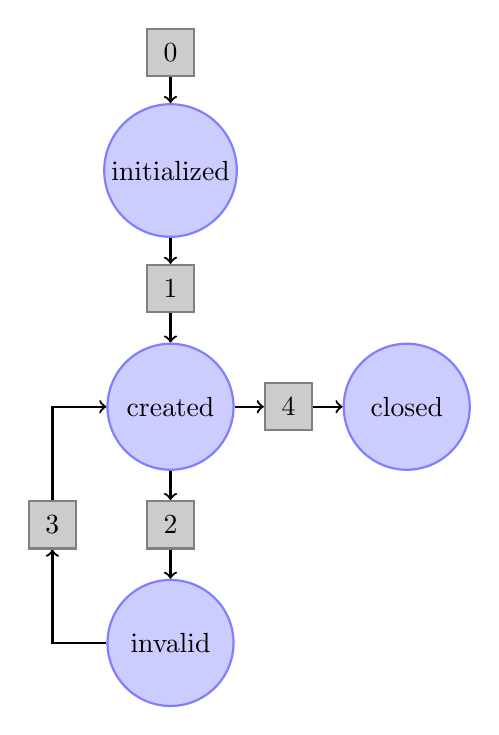
\begin{tikzpicture}
  [state/.style={circle, minimum size=16mm, 
  				node distance=1.5cm, inner sep=2pt, pin distance=4mm, 
  				draw=blue!50,fill=blue!20,thick
                },
   action/.style={rectangle, minimum size=6mm, 
  				node distance=1.5cm, inner sep=2pt, pin distance=4mm, 
  				draw=black!50,fill=black!20,thick
                }
                  ]
  \node[action] (a0) {0};
  \node[state] (init) [below of=a0]{initialized};
  \node[action] (a1) [below of=init]{1};
  \node[state] (cr) [below of=a1]{created};
  \node[action] (a2) [below of=cr]{2};
  \node[action] (a4) [right of=cr]{4};
  \node[state] (cl) [right of=a4]{closed};
  \node[state] (inv) [below of=a2]{invalid};
  \node[action] (a3) [left of=a2]{3};
  \draw[->, thick] (a0.south) -- (init.north);
  \draw[->, thick] (init.south) -- (a1.north);
  \draw[->, thick] (a1.south) -- (cr.north);
  \draw[->, thick] (cr.south) -- (a2.north);
  \draw[->, thick] (a2.south) -- (inv.north);
  \draw[->, thick] (inv.west) -| (a3.south);
  \draw[->, thick] (a3.north) |- (cr.west);
  \draw[->, thick] (cr.east) -- (a4.west);
  \draw[->, thick] (a4.east) -- (cl.west);
\end{tikzpicture}
\caption[Stany zlecenia]{Stany zlecenia. 0 -- utworzenie katalogu na nowe
zlecenie; 1 -- utworzenie pliku ,,body.xml''; 2 -- utworzenie pliku ,,comments.xml''; 3 --
skasowanie pliku ,,comments.xml''; 4 -- utworzenie pliku ,,response.dicom''.}
\label{fig:stany_zlec}
\end{figure}

Serwer, będący de facto serwerem plików z ustaloną sztywno strukturą katalogową, nie
analizuje swojego stanu, jest to zadanie dla klienta i interfejsu konsultanta. Możliwe
stany dla zlecenia przedstawia rysunek \ref{fig:stany_zlec}. Przejścia między stanami
wywoływane są pojawianiem się (lub znikaniem) plików. W zależności od sposobu realizacji
wykrywania zmian, koniecznym może być zapewnienie atomowości operacji dodawania pliku
do struktury. Zmiana stanu MUSI następować dopiero po pojawieniu się w strukturze
kompletnego pliku.

Komentarz do poszczególnych stanów:

\subsection{Lista usług}

Konsultant MUSI udostępnić listę oferowanych usług. Lista zdefiniowanych usług jest
trzymana na serwerze w pliku \textit{/medeos/order/\textbf{services}}. Jest to plik XML,
którego format został określony w sekcji \ref{sec:formaty}. Zleceniodawca, tworząc treść
zlecenia, wpisuje w jego treść nazwę wybranej usługi pobraną z pliku z listą usług. Jeśli
na serwerze pojawi się zlecenie z nazwą usługi nie występującą na liście usług to
konsultant (lub serwer automatycznie) powinien zgłosić w komentarzu konieczność poprawy
zlecenia. W praktyce zwykle usługi będą odpowiadać opisywanym typom badań.


\section{Bezpieczeństwo}
\label{sec:bezp}

Bezpieczeństwo jest realizowane na czterech poziomach: uwierzytelnianie klienta na
serwerze, autoryzacja, poufność transmisji oraz podpis elektroniczny
zlecenia i opisu. Do uwierzytelniania i poufności POWINNO zostać użycie HTTPS i certyfikaty
X.509. Jest to rozwiązanie o wysokim stopniu bezpieczeństwa i łatwe do implementacji.

\subsection{Uwierzytelnianie klienta} 

Celem uwierzytelniania klienta jest zabezpieczenie danych przed dostępem osób
nieupoważnionych oraz możliwość jednoznacznego powiązania przesłanego zlecenia z
instytucją, która je przysłała. Uwierzytelnianie klienta jest zależne od metody transportu
plików. Może bazować na certyfikatach lub loginie i haśle. Zalecane jest użycie
certyfikatów i protokołu HTTPS.

\subsection{Autoryzacja}

Autoryzacja ma na celu zabezpieczenie danych przed dostępem osób nieupoważnionych oraz
zabezpieczenie przed uszkodzeniem struktury danych na serwerze. W przypadku użycia
HTTP$[$S$]$ jako metody transportowej, autoryzacja klienta może być realizowana przez sam
serwer HTTP lub przez CGI obsługujące metody GET, PUT i DELETE. Podstawowa weryfikacja
polega na porównaniu CN z certyfikatu klienta z nazwą klienta zawartą w URL zlecenia.
Serwer POWINIEN mieć również możliwość dodawania kolejnych CN do listy uprawnionych do
dostępu do danego katalogu ze zleceniem. Niezależnie od metody transportowej autoryzację
można realizować przez kontrolę dostępu wbudowaną w system plików. W praktyce stosowana
będzie kombinacja tych opcji. Dostęp po poszczególnych zasobów przedstawia się następująco:
\begin{description}
  \item[/medeos/order/$<$\textit{client}$>$/]\hfill\\
  Dostęp do całego katalogu ma jeden określony klient oraz interfejs konsultanta. Klient
  może tutaj zapisywać i czytać, konsultant tylko czytać.
  \item[/medeos/order/$<$\textit{client}$>$/$<$\textit{order id}$>$/response/]\hfill\\ 
  W tym katalogu interfejs konsultanta może zapisywać.
  \item[/medeos/order/$<$\textit{client}$>$/$<$\textit{order id}$>$/history/]\hfill\\ 
  W tym katalogu zapisywać może serwer lub interfejs konsultanta.
\end{description}

\subsection{Poufność transmisji}

Poufność transmisji POWINNA być zapewniona poprzez zastosowanie odpowiednich algorytmów
szyfrujących przesyłane dane. Zalecane jest użycie algorytmu AES z kluczem co najmniej 128
bitów. Do tego celu zaleca się użycie protokołu HTTPS z konfiguracją serwera zezwalającą
na połączenia tylko z użyciem AES 128 bit lub lepszym. W przypadku użycia do transportu
plików protokołu, który nie zapewnia szyfrowania, poufność należy zapewnić poprzez
zastosowanie szyfrowanych tuneli lub sieci VPN.

\subsection{Podpis elektroniczny}
\label{sec:sig}

Opcjonalnie zleceniodawca i konsultant mogą się zdecydować na użycie podpisu
elektronicznego w celu potwierdzenia autorstwa i integralności danych. Podpis elektroniczny
nie jest niezbędny dla działania Systemu, stanowi jedynie zabezpieczenie dla komunikujących
się stron w sprawach spornych. Strony, które nie obsługują podpisów MUSZĄ ignorować pliki
zawierające podpisy. Dla zwiększenia przezroczystości podpisy są realizowane w postaci
\emph{DETACHED}, czyli są przechowywane w osobnych plikach niezależnie od plików z danymi.
Nazwa pliku z podpisem tworzona jest poprzez dodanie odpowiedniego rozszerzenia do nazwy
pliku podpisywanego. Rozszerzenie jest zależne od użytego formatu zapisu podpisu.
Dopuszczone są następujące postaci podpisów:
\begin{description}
  \item[W3C xmldsig-core 20080610] -- rozszerzenie \textit{.xmldsig.xml}
  \item[W3C XAdES 20030220] -- rozszerzenie \textit{.xades.xml}
  \item[ETSI TS 101 903 V1.3.2] -- rozszerzenie \textit{.etsi-ts-101-903.xml}
\end{description}

ZALECA się użycie formatu \textit{XAdES} lub \textit{ETSI TS 101 903}.

Plik z podpisem musi zawierać URI oraz sumy kontrolne podpisywanych plików oraz certyfikat
X509v3 podpisującego, umożliwiający weryfikację podpisu (zawierający klucz publiczny
powiązany z kluczem prywatnym użytym do podpisu).

Podpisywane są tylko wybrane pliki i są to: \emph{body.xml} -- treść zlecenia,
\emph{response.dicom} -- opis i \emph{comments.xml} -- komentarz konsultanta, plus ew.
załączniki do nich. Załączniki są podpisywane razem z plikiem wiodącym którego dotyczą,
poprzez użycie dodatkowych elementów \emph{Reference}.

Po każdej zmianie w podpisanym pliku należy przygotować nowy podpis i umieścić go na
serwerze. Dotyczy to również zmian w załącznikach. Podmieniane pliki wraz z ich podpisami
MUSZĄ być przenoszone do historii.

Jeśli katalog z podpisanym zleceniem lub katalog z podpisanym opisem zawiera niepodpisane
pliki, to uznaje się, że weryfikacja podpisu nie powiodła się. Jeśli weryfikacja podpisu 

\subsubsection{Wiązanie plików przy xmldsig-core}

Wiązanie plików jest realizowane poprzez stworzenie wielu instancji \emph{Reference} w
obiekcie \emph{SignedInfo}. Atrybut URI MUSI wskazywać na pełen adres URL wskazujący
na plik, którego dotyczy wymieniony w \emph{DigestValue} skrót.

\subsubsection{Wiązanie plików przy ETSI TS 101 903}

Analogicznie jak dla \emph{xmldsig-core}.

\subsubsection{Wiązanie plików przy XAdES}

Analogicznie jak dla \emph{xmldsig-core}.

\subsubsection{Znakowanie czasem}

System przewiduje możliwość znakowania czasem tworzonych plików w połączeniu z podpisem
elektronicznym w postaci XML. Standardy \textit{XAdES} i \textit{ETSI TS 101 903}
określają możliwe metody znakowania podpisu czasem i należy postępować zgodnie z zasadami
opisanymi w tych standardach. 

W przypadku nie używania Time-Stamp Protocol (RFC 3161) należy w obiekcie \emph{Object}
utworzyć element \emph{SignatureTime} wypełniony datą i czasem dokonania podpisu zapisanym w
formacie ISO 8601 i dodać obiekt \emph{Reference} wskazujący na \emph{Object} zawierający
\emph{SignatureTime}. Podpisujący deklaruje, że podpis został wykonany nie wcześniej niż o
godzinie wpisanej w \emph{SignatureTime}. Druga strona (weryfikująca znacznik czasu)
obowiązana jest do zweryfikowania czasu podanego w \emph{SignatureTime}. Weryfikacja
POWINNA odbywać się automatycznie zgodnie z polityką jednotski korzystającej z Sytemu. W
razie zastrzeżeń co do wpisanego czasu, należy niezwłocznie powiadomić drugą stronę o
zaistniałym problemie.

Znakowanie czasem nie jest niezbędne dla działania Systemu, stanowi jedynie
zabezpieczenie dla komunikujących się stron w sprawach spornych.

Do znakowania czasem zalecane jest użycie Time-Stamp Protocol (RFC 3161) w połączeniu z
podpisem w formacie \textit{XAdES} lub \textit{ETSI TS 101 903}.

\subsubsection{Potwierdzenie przyjęcia zlecenia}

Gdy para klient-serwer decyduje się na użycie podpisu elektronicznego, to serwer MUSI
tworzyć podpis elektroniczny potwierdzający przyjęcie zlecenia. Podpis ten podpisuje plik z
podpisem zleceniodawcy. Jest to plik \emph{confirm.$<$\textit{sig\_ext}$>$} opisany w
sekcji \ref{sec:model}. Podpis MUSI być tworzony automatycznie, niezwłocznie po otrzymaniu
kompletnego zlecenia przez serwer. Podpis potwierdzający przyjęcie zlecenia MUSI zawierać
datę wykonania podpisu. Może być to data zapisana w elemencie \emph{SignatureTime} lub
znacznik czasu dla podpisu otrzymany z serwera obsługując RFC 3161 i zapisany zgodnie z
\textit{XAdES} lub \textit{ETSI TS 101 903}.

\subsection{Historia zlecenia}
\label{sec:hist}

Zmodyfikowane lub skasowane pliki stanowiące treść zlecenia nie są tracone bezpowrotnie.
Serwer MUSI przenosić usuwany plik do katalogu\\
\textbf{/medeos/order/$<$\textit{client}$>$/$<$\textit{order id}$>$/history/}.
Nazwa przenoszonego pliku jest budowana poprzez dodanie daty i godziny modyfikacji do
oryginalnej nazwy. Czas POWINIEN być zapisywany w formacie zgodnym z ISO (YYYY-MM-DDThh:mm:ss.sTZD)

\section{Formaty plików}
\label{sec:formaty}

System ingeruje w treść tylko jednego pliku, tj. pliku \newline
,,/medeos/order/$<$\textit{client}$>$/$<$\textit{order id}$>$/history/log''. \newline Treść
pozostałych plików jest interpretowana jedynie przez interfejsy użytkownika. Aby zapewnić
interoperacyjność między interfejsami zleceniodawcy i konsultanta, formaty plików ze
zleceniem, opisem i komentarzem muszą zostać ustalone. 

Poniżej ogólne ustalenia co do formatu XML.
\begin{itemize}
  \item Wszystkie pliki w formacie XML MUSZĄ mieć kodowanie znaków w standardzie UTF-8.
  \item Plik NIE MOŻE zawierać znacznika UTF BOM.
  \item Ciągi białych znaków bezpośrednio za znacznikiem otwierającym element oraz
  bezpośrednio przed znacznikiem zamykającym element POWINNY być ignorowane. 
\end{itemize}
 
Interfejs zleceniodawcy oraz interfejs konsultanta MUSZĄ obsługiwać załączniki w formacie
DICOM. Dozwolone jest przesyłanie załączników również w innych formatach. Jeśli
zleceniodawca wyśle załącznik w formacie nieobsługiwanym przez serwer, to serwer POWINIEN
automatycznie wystawić komentarz z informacją o nieobsługiwanym formacie pliku.

\subsection{Format pliku ze zleceniem}

Zlecenie jest dokumentem XML o następującej strukturze:

\noindent
\ttfamily
\hlstd{}\hlkwa{$<$?xml\ }\hlstd{}\hlkwb{version}\hlstd{=}\hlstr{"1.0"}\hlstd{\ }\hlkwb{encoding}\hlstd{=}\hlstr{"UTF{-}8"}\hlstd{}\hlkwa{?$>$}\hspace*{\fill}\\
\hlstd{}\hlkwa{$<$Medeos\ }\hlstd{}\hlkwb{xmlns}\hlstd{=}\hlstr{"http://www.medeos.org/v1.0"}\hlstd{}\hlkwa{$>$}\hspace*{\fill}\\
\hlstd{\ }\hlkwa{$<$Order\ }\hlstd{}\hlkwb{created}\hlstd{=}\hlstr{"czas\ utworzenia\ dokumentu\ przez\ klienta"}\hlstd{}\hlkwa{$>$}\hspace*{\fill}\\
\hlstd{}\hlstd{\ \ }\hlstd{}\hlkwa{$<$Sender$>$}\hspace*{\fill}\\
\hlstd{}\hlstd{\ \ \ }\hlstd{}\hlkwa{$<$UnitName$>$}\hspace*{\fill}\\
\hlstd{}\hlstd{\ \ \ \ }\hlstd{Nazwa\ jednostki\ wysyłającej\ komunikat.\hspace*{\fill}\\
}\hlstd{\ \ \ \ }\hlstd{Najlepiej\ CN\ z\ cetryfikatu\ lub\ jego\ fragment\hspace*{\fill}\\
}\hlstd{\ \ \ }\hlstd{}\hlkwa{$<$/UnitName$>$}\hspace*{\fill}\\
\hlstd{}\hlstd{\ \ \ }\hlstd{}\hlkwa{$<$StationName$>$}\hspace*{\fill}\\
\hlstd{}\hlstd{\ \ \ \ }\hlstd{Nazwa\ stacji\ wysyłającej\ komunikat.\hspace*{\fill}\\
}\hlstd{\ \ \ \ }\hlstd{Najlepiej\ CN\ z\ cetryfikatu\ lub\ jego\ fragment\hspace*{\fill}\\
}\hlstd{\ \ \ }\hlstd{}\hlkwa{$<$/StationName$>$}\hspace*{\fill}\\
\hlstd{}\hlstd{\ \ \ }\hlstd{}\hlkwa{$<$Person$>$}\hlstd{}\hlcom{$<$!{-}{-}\ Dane\ o\ wysyłającym\ powinny\ być}\hspace*{\fill}\\
\hlcom{}\hlstd{\ \ \ \ \ \ }\hlcom{weryfikowane\ względem\ podpisiu\ elektronicznego\ {-}{-}$>$}\hlstd{\hspace*{\fill}\\
}\hlstd{\ \ \ \ }\hlstd{}\hlkwa{$<$Name$>$}\hlstd{Nazwa\ osoby\ wysyłającej\ komunikat.}\hlkwa{$<$/Name$>$}\hspace*{\fill}\\
\hlstd{}\hlstd{\ \ \ \ }\hlstd{}\hlkwa{$<$Licence$>$}\hlstd{Opcjonalny\ numer\ prawa\ wykonywania\ zawodu\hspace*{\fill}\\
}\hlstd{\ \ \ \ \ \ \ }\hlstd{lekarza\ zlecającego.\hspace*{\fill}\\
}\hlstd{\ \ \ \ }\hlstd{}\hlkwa{$<$/Licence$>$}\hspace*{\fill}\\
\hlstd{}\hlstd{\ \ \ \ }\hlstd{}\hlkwa{$<$EMail$>$}\hlstd{Adres\ e{-}mail\ do\ powiadomień.}\hlkwa{$<$/EMail$>$}\hspace*{\fill}\\
\hlstd{}\hlstd{\ \ \ \ }\hlstd{}\hlkwa{$<$Phone$>$}\hlstd{Telefon\ kontaktowy.}\hlkwa{$<$/Phone$>$}\hspace*{\fill}\\
\hlstd{}\hlstd{\ \ \ }\hlstd{}\hlkwa{$<$/Person$>$}\hspace*{\fill}\\
\hlstd{}\hlstd{\ \ \ }\hlstd{}\hlkwa{$<$AdditionalContactInfo$>$\ }\hlstd{}\hlcom{$<$!{-}{-}\ opcjonalne\ {-}{-}$>$}\hlstd{\hspace*{\fill}\\
}\hlstd{\ \ \ \ }\hlstd{Tekst\ z\ uwagami\ na\ temat\ możliwości\ kontaktu\ ze\ zleceniodawcą.\hspace*{\fill}\\
}\hlstd{\ \ \ }\hlstd{}\hlkwa{$<$/AdditionalContactInfo$>$}\hspace*{\fill}\\
\hlstd{}\hlstd{\ \ }\hlstd{}\hlkwa{$<$/Sender$>$}\hspace*{\fill}\\
\hlstd{}\hlstd{\ \ }\hlstd{}\hlkwa{$<$Receiver$>$}\hspace*{\fill}\\
\hlstd{}\hlstd{\ \ \ }\hlstd{}\hlkwa{$<$UnitName$>$}\hspace*{\fill}\\
\hlstd{}\hlstd{\ \ \ \ }\hlstd{Nazwa\ jednostki,\ która\ ma\ sie\ zająć\hspace*{\fill}\\
}\hlstd{\ \ \ \ }\hlstd{realizacją\ zlecenia.\hspace*{\fill}\\
}\hlstd{\ \ \ }\hlstd{}\hlkwa{$<$/UnitName$>$}\hspace*{\fill}\\
\hlstd{}\hlstd{\ \ \ }\hlstd{}\hlkwa{$<$PersonName$>$}\hspace*{\fill}\\
\hlstd{}\hlstd{\ \ \ \ }\hlstd{Opcjonalna\ nazwa\ osoby,\ która\ ma\ się\hspace*{\fill}\\
}\hlstd{\ \ \ \ }\hlstd{zająć\ realizacją\ zlecenia.\hspace*{\fill}\\
}\hlstd{\ \ \ }\hlstd{}\hlkwa{$<$/PersonName$>$}\hspace*{\fill}\\
\hlstd{}\hlstd{\ \ }\hlstd{}\hlkwa{$<$/Receiver$>$}\hspace*{\fill}\\
\hlstd{}\hlstd{\ \ }\hlstd{}\hlkwa{$<$Patient\ }\hlstd{}\hlkwb{id}\hlstd{=}\hlstr{"unikalny\ identyfikator\ pacjenta\ nadawany\ przez\ klienta}\hspace*{\fill}\\
\hlstr{}\hlstd{\ \ \ \ \ \ }\hlstr{(np.\ pesel)"}\hlstd{}\hlkwa{$>$}\hspace*{\fill}\\
\hlstd{}\hlstd{\ \ \ }\hlstd{}\hlkwa{$<$Name$>$}\hlstd{Nazwa\ pacjenta\ lub\ }\hlstr{"Pacjent\ Anonimowy"}\hlstd{.}\hlkwa{$<$/Name$>$}\hspace*{\fill}\\
\hlstd{}\hlstd{\ \ \ }\hlstd{}\hlkwa{$<$Gender$>$}\hlstd{Płeć\ pacjenta:\ male\textbar female\textbar unidentified}\hlkwa{$<$/Gender$>$}\hspace*{\fill}\\
\hlstd{}\hlstd{\ \ \ }\hlstd{}\hlkwa{$<$DateOfBirth$>$}\hspace*{\fill}\\
\hlstd{}\hlstd{\ \ \ \ \ \ \ }\hlstd{}\hlkwa{$<$Month$>$}\hlstd{}\hlnum{1}\hlstd{}\hlkwa{$<$/Month$>$}\hlstd{}\hlcom{$<$!{-}{-}\ Opcjonalne\ {-}{-}$>$}\hlstd{\hspace*{\fill}\\
}\hlstd{\ \ \ \ \ \ \ \ \ }\hlstd{}\hlkwa{$<$Day$>$}\hlstd{}\hlnum{15}\hlstd{}\hlkwa{$<$/Day$>$}\hlstd{}\hlcom{$<$!{-}{-}\ Opcjonalne\ {-}{-}$>$}\hlstd{\hspace*{\fill}\\
}\hlstd{\ \ \ \ \ \ \ \ \ }\hlstd{}\hlkwa{$<$Year$>$}\hlstd{}\hlnum{2001}\hlstd{}\hlkwa{$<$/Year$>$}\hspace*{\fill}\\
\hlstd{}\hlstd{\ \ \ }\hlstd{}\hlkwa{$<$/DateOfBirth$>$}\hspace*{\fill}\\
\hlstd{}\hlstd{\ \ \ }\hlstd{}\hlkwa{$<$Address$>$}\hlstd{}\hlcom{$<$!{-}{-}\ Opcjonalne\ {-}{-}$>$}\hlstd{\hspace*{\fill}\\
}\hlstd{\ \ \ \ \ \ \ \ \ \ }\hlstd{}\hlkwa{$<$Street1$>$$<$/Street1$>$}\hspace*{\fill}\\
\hlstd{}\hlstd{\ \ \ \ \ \ \ \ \ \ }\hlstd{}\hlkwa{$<$Street2$>$$<$/Street2$>$}\hspace*{\fill}\\
\hlstd{}\hlstd{\ \ \ \ \ \ \ \ \ \ }\hlstd{}\hlkwa{$<$City$>$$<$/City$>$}\hspace*{\fill}\\
\hlstd{}\hlstd{\ \ \ \ \ \ \ \ \ \ }\hlstd{}\hlkwa{$<$Zip$>$$<$/Zip$>$}\hspace*{\fill}\\
\hlstd{}\hlstd{\ \ \ \ \ \ \ \ \ \ }\hlstd{}\hlkwa{$<$Region$>$$<$/Region$>$}\hspace*{\fill}\\
\hlstd{}\hlstd{\ \ \ \ \ \ \ \ \ \ }\hlstd{}\hlkwa{$<$Country$>$$<$/Country$>$}\hspace*{\fill}\\
\hlstd{}\hlstd{\ \ \ }\hlstd{}\hlkwa{$<$/Address$>$}\hspace*{\fill}\\
\hlstd{}\hlstd{\ \ }\hlstd{}\hlkwa{$<$/Patient$>$}\hspace*{\fill}\\
\hlstd{}\hlstd{\ \ }\hlstd{}\hlkwa{$<$RequestedService\ }\hlstd{}\hlkwb{id}\hlstd{=}\hlstr{"id\ ze\ słownika\ usług"}\hlstd{}\hlkwa{$>$}\hspace*{\fill}\\
\hlstd{}\hlstd{\ \ \ }\hlstd{}\hlkwa{$<$Priority\ }\hlstd{}\hlkwb{value}\hlstd{=}\hlstr{"wartość\ 0{-}2;\ 0\ {-}\ niski,\ 1\ {-}\ normalny,\ 2\ {-}\ pilny"}\hlstd{}\hlkwa{/$>$}\hspace*{\fill}\\
\hlstd{}\hlstd{\ \ \ }\hlstd{}\hlcom{$<$!{-}{-}\ Priority\ wpływa\ między\ innymi\ na\ kolejkowanie\ wysyłanych\ zleceń}\hspace*{\fill}\\
\hlcom{}\hlstd{\ \ \ }\hlcom{po\ stronie\ klienta\ {-}{-}$>$}\hlstd{\hspace*{\fill}\\
}\hlstd{\ \ \ }\hlstd{}\hlkwa{$<$Description$>$}\hlstd{Rozpoznanie}\hlkwa{$<$/Description$>$}\hspace*{\fill}\\
\hlstd{}\hlstd{\ \ \ }\hlstd{}\hlkwa{$<$Problem$>$}\hlstd{Co\ badanie\ ma\ wyjaśnić}\hlkwa{$<$/Problem$>$}\hspace*{\fill}\\
\hlstd{}\hlstd{\ \ \ }\hlstd{}\hlkwa{$<$Comment$>$}\hlstd{Komentarz}\hlkwa{$<$/Comment$>$}\hspace*{\fill}\\
\hlstd{}\hlstd{\ \ }\hlstd{}\hlkwa{$<$/RequestedService$>$}\hspace*{\fill}\\
\hlstd{\ }\hlkwa{$<$/Order$>$}\hspace*{\fill}\\
\hlstd{}\hlkwa{$<$/Medeos$>$}\hlstd{}\hspace*{\fill}\\
\mbox{}
\normalfont


\subsection{Format pliku z komentarzem}

Komentarz jest dokumentem XML o następującej strukturze:

\noindent
\ttfamily
\hlstd{}\hlkwa{$<$?xml\ }\hlstd{}\hlkwb{version}\hlstd{=}\hlstr{"1.0"}\hlstd{\ }\hlkwb{encoding}\hlstd{=}\hlstr{"UTF{-}8"}\hlstd{}\hlkwa{?$>$}\hspace*{\fill}\\
\hlstd{}\hlkwa{$<$Medeos\ }\hlstd{}\hlkwb{xmlns}\hlstd{=}\hlstr{"http://www.medeos.org/v1.0"}\hlstd{}\hlkwa{$>$}\hspace*{\fill}\\
\hlstd{\ }\hlkwa{$<$ConsultantsComments\ }\hlstd{}\hlkwb{created}\hlstd{=}\hlstr{"czas\ utworzenia\ dokumentu"}\hlstd{}\hlkwa{$>$}\hspace*{\fill}\\
\hlstd{}\hlstd{\ \ }\hlstd{}\hlkwa{$<$Author$>$}\hspace*{\fill}\\
\hlstd{}\hlstd{\ \ \ }\hlstd{}\hlkwa{$<$UnitName$>$}\hspace*{\fill}\\
\hlstd{}\hlstd{\ \ \ \ }\hlstd{Nazwa\ jednostki\ wysyłającej\ komunikat.\hspace*{\fill}\\
}\hlstd{\ \ \ \ }\hlstd{Najlepiej\ CN\ z\ cetryfikatu\ lub\ jego\ fragment\hspace*{\fill}\\
}\hlstd{\ \ \ }\hlstd{}\hlkwa{$<$/UnitName$>$}\hspace*{\fill}\\
\hlstd{}\hlstd{\ \ \ }\hlstd{}\hlkwa{$<$Person$>$}\hlstd{}\hlcom{$<$!{-}{-}\ Docelowo\ dane\ o\ wysyłającym\ mają\ być}\hspace*{\fill}\\
\hlcom{}\hlstd{\ \ \ \ \ \ }\hlcom{weryfikowane\ względem\ podpisiu\ elektronicznego\ {-}{-}$>$}\hlstd{\hspace*{\fill}\\
}\hlstd{\ \ \ \ }\hlstd{}\hlkwa{$<$Name$>$}\hlstd{Nazwa\ osoby\ wysyłającej\ komunikat.}\hlkwa{$<$/Name$>$}\hspace*{\fill}\\
\hlstd{}\hlstd{\ \ \ \ }\hlstd{}\hlkwa{$<$Licence$>$}\hlstd{Opcjonalny\ numer\ prawa\ wykonywania\ zawodu\hspace*{\fill}\\
}\hlstd{\ \ \ \ \ \ }\hlstd{lekarza\ zlecającego.\hspace*{\fill}\\
}\hlstd{\ \ \ \ }\hlstd{}\hlkwa{$<$/Licence$>$}\hspace*{\fill}\\
\hlstd{}\hlstd{\ \ \ }\hlstd{}\hlkwa{$<$/Person$>$}\hspace*{\fill}\\
\hlstd{}\hlstd{\ \ }\hlstd{}\hlkwa{$<$/Author$>$}\hspace*{\fill}\\
\hlstd{}\hlstd{\ \ }\hlstd{}\hlkwa{$<$Summary$>$}\hspace*{\fill}\\
\hlstd{}\hlstd{\ \ \ }\hlstd{Krótkie\ podsumowanie.\hspace*{\fill}\\
}\hlstd{\ \ }\hlstd{}\hlkwa{$<$/Summary$>$}\hspace*{\fill}\\
\hlstd{}\hlstd{\ \ }\hlstd{}\hlkwa{$<$Body$>$}\hspace*{\fill}\\
\hlstd{}\hlstd{\ \ \ }\hlstd{Treść\ komentarza.\hspace*{\fill}\\
}\hlstd{\ \ }\hlstd{}\hlkwa{$<$/Body$>$}\hspace*{\fill}\\
\hlstd{}\hlstd{\ \ }\hlstd{}\hlkwa{$<$InResponseTo$>$}\hspace*{\fill}\\
\hlstd{}\hlstd{\ \ \ }\hlstd{}\hlkwa{$<$Order\ }\hlstd{}\hlkwb{sha256}\hlstd{=}\hlstr{"befdf0df30cd0943c828a3b54d058067a20931a9cc0f409b3dc8aa56d342179e"}\hlstd{}\hlkwa{/$>$}\hspace*{\fill}\\
\hlstd{}\hlstd{\ \ }\hlstd{}\hlkwa{$<$/InResponseTo$>$}\hspace*{\fill}\\
\hlstd{\ }\hlkwa{$<$/ConsultantsComments$>$}\hspace*{\fill}\\
\hlstd{}\hlkwa{$<$/Medeos$>$}\hlstd{}\hspace*{\fill}\\
\mbox{}
\normalfont


\subsection{Format pliku z logiem servera}

,,Log'' jest dokumentem XML o następującej strukturze:

\noindent
\ttfamily
\hlstd{}\hlkwa{$<$?xml\ }\hlstd{}\hlkwb{version}\hlstd{=}\hlstr{"1.0"}\hlstd{\ }\hlkwb{encoding}\hlstd{=}\hlstr{"UTF{-}8"}\hlstd{}\hlkwa{?$>$}\hspace*{\fill}\\
\hlstd{}\hlkwa{$<$Medeos\ }\hlstd{}\hlkwb{xmlns}\hlstd{=}\hlstr{"http://www.medeos.org/v1.0.0"}\hlstd{}\hlkwa{$>$}\hspace*{\fill}\\
\hlstd{\ }\hlkwa{$<$Log$>$}\hspace*{\fill}\\
\hlstd{}\hlstd{\ \ }\hlstd{}\hlkwa{$<$Entry\ }\hlstd{}\hlkwb{time}\hlstd{=}\hlstr{"czas\ wpisu"}\hlstd{\ }\hlkwb{module}\hlstd{=}\hlstr{"nazwa\ komponentu\ dokonującego\ wpisu"}\hlstd{\hspace*{\fill}\\
}\hlstd{\ \ \ \ }\hlstd{}\hlkwb{priority}\hlstd{=}\hlstr{"DEBUG\textbar INFO\textbar NOTICE\textbar WARN\textbar ERROR\textbar CRITICAL"}\hlstd{}\hlkwa{$>$}\hspace*{\fill}\\
\hlstd{}\hlstd{\ \ \ }\hlstd{}\hlcom{$<$!{-}{-}\ jedno\ z\ dwóch\ poniższych\ {-}{-}$>$}\hlstd{\hspace*{\fill}\\
}\hlstd{\ \ \ }\hlstd{}\hlkwa{$<$File\ }\hlstd{}\hlkwb{name}\hlstd{=}\hlstr{""}\hlstd{\ }\hlkwb{changeType}\hlstd{=}\hlstr{"PUT\textbar DELETE"}\hlstd{}\hlkwa{$>$}\hspace*{\fill}\\
\hlstd{}\hlstd{\ \ \ \ }\hlstd{Opis\ zmiany.\hspace*{\fill}\\
}\hlstd{\ \ \ }\hlstd{}\hlkwa{$<$/File$>$}\hspace*{\fill}\\
\hlstd{}\hlstd{\ \ \ }\hlstd{}\hlkwa{$<$Message$>$}\hspace*{\fill}\\
\hlstd{}\hlstd{\ \ \ \ }\hlstd{Treść\ wiadomości.\hspace*{\fill}\\
}\hlstd{\ \ \ }\hlstd{}\hlkwa{$<$/Message$>$}\hspace*{\fill}\\
\hlstd{}\hlstd{\ \ }\hlstd{}\hlkwa{$<$/Entry$>$}\hspace*{\fill}\\
\hlstd{}\hlstd{\ \ }\hlstd{...\hspace*{\fill}\\
\ }\hlkwa{$<$/Log$>$}\hspace*{\fill}\\
\hlstd{}\hlkwa{$<$/Medeos$>$}\hlstd{}\hspace*{\fill}\\
\mbox{}
\normalfont


\subsection{Format pliku z listą usług}

,,Services'' jest dokumentem XML o następującej strukturze:

\noindent
\ttfamily
\hlstd{}\hlkwa{$<$?xml\ }\hlstd{}\hlkwb{version}\hlstd{=}\hlstr{"1.0"}\hlstd{\ }\hlkwb{encoding}\hlstd{=}\hlstr{"UTF{-}8"}\hlstd{}\hlkwa{?$>$}\hspace*{\fill}\\
\hlstd{}\hlkwa{$<$Medeos\ }\hlstd{}\hlkwb{xmlns}\hlstd{=}\hlstr{"http://www.medeos.org/v1.0.0"}\hlstd{}\hlkwa{$>$}\hspace*{\fill}\\
\hlstd{\ }\hlkwa{$<$Services$>$}\hspace*{\fill}\\
\hlstd{}\hlstd{\ \ }\hlstd{}\hlkwa{$<$Service$>$}\hspace*{\fill}\\
\hlstd{}\hlstd{\ \ \ }\hlstd{}\hlkwa{$<$Name$>$}\hlstd{Nazwa\ serwisu.\ Nazwa\ serwisu\ jest\ jednocześnie\ jego\hspace*{\fill}\\
}\hlstd{\ \ \ \ }\hlstd{identyfikatorem\ i\ pojawia\ się\ w\ zleceniu\ (plik\ body).\hspace*{\fill}\\
}\hlstd{\ \ \ }\hlstd{}\hlkwa{$<$/Name$>$}\hspace*{\fill}\\
\hlstd{}\hlstd{\ \ \ }\hlstd{}\hlkwa{$<$Description$>$}\hspace*{\fill}\\
\hlstd{}\hlstd{\ \ \ \ }\hlstd{Opis\ serwisu.\hspace*{\fill}\\
}\hlstd{\ \ \ }\hlstd{}\hlkwa{$<$/Description$>$}\hspace*{\fill}\\
\hlstd{}\hlstd{\ \ }\hlstd{}\hlkwa{$<$/Service$>$}\hspace*{\fill}\\
\hlstd{}\hlstd{\ \ }\hlstd{...\hspace*{\fill}\\
\ }\hlkwa{$<$/Services$>$}\hspace*{\fill}\\
\hlstd{}\hlkwa{$<$/Medeos$>$}\hlstd{}\hspace*{\fill}\\
\mbox{}
\normalfont


\end{document}
